\documentclass[CJK,11pt]{amsart}
\usepackage{CJK}
\usepackage{lipsum}
\usepackage{amsfonts}
\usepackage{graphicx}
\usepackage{epstopdf}
\usepackage{algorithmic}
\usepackage{hyperref}
\hypersetup{
	colorlinks=true,
	linkcolor=blue,
	filecolor=blue,      
	urlcolor=blue,
	citecolor=cyan,
}
\ifpdf
  \DeclareGraphicsExtensions{.eps,.pdf,.png,.jpg}
\else
  \DeclareGraphicsExtensions{.eps}
\fi

% Add a serial/Oxford comma by default.
\newcommand{\creflastconjunction}{, and~}

\usepackage{amsopn}
\DeclareMathOperator{\diag}{diag}


\usepackage{relsize}
\usepackage{pxfonts}
\usepackage{tikz}
\usetikzlibrary{arrows,shapes,chains,positioning}
\usetikzlibrary{decorations.markings}
\tikzstyle arrowstyle=[scale=1]
\tikzstyle directed=[postaction={decorate,decoration={markings,mark=at position .65 with {\arrow[arrowstyle]{stealth}}}}]
\tikzstyle reverse directed=[postaction={decorate,decoration={markings,mark=at position .65 with {\arrowreversed[arrowstyle]{stealth};}}}]
\newtheorem{Def}{Definition}
\newtheorem{Th}{Theorem}[section]
\newtheorem{Lm}{Lemma}[section] 
  
\theoremstyle{definition}

\begin{document}
\begin{CJK*}{UTF8}{gbsn}
%  \title{Dedicated to the Memory of My Mentor Jim Bramble}
  \title{ In Loving Memory of My Great Mentor Jim Bramble}
\author{Jinchao Xu}
\begin{abstract}
Jim Bramble was one of the most distinguished computational mathematicians of all time. He made many fundamental contributions to the design and analysis of numerical methods for partial differential equations, including the finite difference method, the finite element method, and the multigrid and domain decomposition methods. He loved mathematics, developed many important algorithms, and proved many great theorems. Yet, he balanced his love of mathematics with a love of life beyond work: He played tennis and golf, knew how to enjoy a good time, and was a true and genuinely caring friend to so many of us. He had a great life! 

Jim was my PhD thesis advisor at Cornell University (spring 1985-fall 1988) where he had made a special effort to get me admitted. He taught me how to conduct high-quality creative research and guided me in many other things in my life. He was a great mentor, a father figure, and a dear friend. His kindness and generosity made an immeasurable impact on me, on my academic career, and on my personal life far beyond that sphere.
I miss him greatly today and know that I will always do so. 
\end{abstract}
\maketitle

James Henry Bramble, one of the most distinguished computational mathematicians of all time, died aged 90 on July 20, 2021, at his home in Austin, Texas. Jim was my PhD thesis advisor at Cornell University (spring 1985-fall 1988). He was a great mentor and dear friend. I miss him greatly today and know that this will never change for me. In this article, I share some recollections about the time I shared with him and the tremendous impact he had on my career and my life more generally. 

\section{First meetings}
Like many researchers working on the finite element method, I first got to know Jim through my reading on the subject. In 1981, as a senior undergraduate student at the Xiangtan University of China, I was working on my senior thesis "Error Estimates of the Finite Element Method for the 2nd Order Elliptic Equation with Discontinuous Coefficients" \cite{xu1982error} when I came across Jim's name for the very first time through the Bramble-Hilbert Lemma, a very basic technique in finite element analysis at the time and still today. 
I first met Jim three years later at the 5th International Conference in Partial Differential Geometries and Partial Differential Equations in Beijing, China, which was started by Professor S.S. Chern and has come to be known as the "Double Partial Conference (双微会议)". The theme of this meeting was numerical methods for partial differential equations, and Jim, an invited speaker, gave the inaugural talk. As a young researcher who was new in a field in which Jim was the world leading authority, I was excited to attend his lecture. I vividly remember him talking about the domain decomposition method, a topic to which he had made fundamental contributions. I recall the way he talked and even the layout of his hand-written slides.

At this time, I had just received my master's degree in mathematics from Peking University, and I, too, was giving a contributed talk at the conference.  My talk was scheduled for the second day. This would be my first-ever talk at a conference and my first-ever in English as well in any public circumstance. After attending Jim's talk, I realized that my slides were not likely to serve me well in sharing my work. I had put too much content on each slide, causing my handwriting to be miniscule. Jim's slides, on the other hand, had very few words, yet the takeaways were crystal clear. Inspired by his talk, I stayed up all night reorganizing my talk and rewriting all my slides. This was the first time that Jim made a meaningful and decisive impact on my work. 

I gave my talk on error estimates for the finite element method the next day, excited and nervous that the world's leading expert on the topic would be sitting in the front row. Near the end of my talk, Jim made some encouraging and complimentary comments. He gave me the impression that he really liked it. After I was done, I mustered up the courage to talk to him. Here I was, a 23-year-old junior researcher at the beginning of my career, speaking broken English, about to approach a giant in my subject from the United States! He greeted me with a huge smile and the kindness in his voice calmed me down. We had a great conversation together --- one of so many more to come. 

\section{Jim took me to Cornell}
In 1983, the Department of Mathematics at Peking University selected six graduate students from all the graduate students entering the school in the year of 1981 and of 1982 to pursue PhD study abroad. I was luckily the one chosen for the field of computational mathematics, as were the now famous mathematicians Tian Gang and Zhang Yitang from other fields. Cornell was my choice and I already applied just before the conference in Beijing.  In my discussion with Jim after my talk, I took the courage to ask him if he could take me on as his graduate student. In response, he had kindly stated that he would be happy to do so and would look into my application. 

True to his word, on returning to Cornell, Jim had done exactly that. But there was a problem: My TOFEL score did not meet the university's minimum requirement. In most circumstances, I could have expected this to kill my chances of gaining admission. But Jim took some extraordinary steps to help me. He contacted the Dean of the Graduate School at Cornell, who, in turn, contacted Ms.~Li Pei (李佩), an English teacher in Beijing well-known for helping students apply to US graduate schools. Next, I found myself at Ms. Li Pei's apartment in ZhongGuanCun (中关村) where,  as a test of my proficiency with the language,  she asked me to write an article in English to explain why and how I came to see her. Luckily, the piece I then produced met with her approval: "Your English writing is quite good. How come you failed the TOFEL exam?" she asked me. She followed up with several more questions in English and Chinese. She then stated that I had passed the test.

With this extraordinary assistance, from Jim, the Dean and Ms. Li, I met the language requirement in this special way. Jim also took another quite unusual step: He made an exception to the well-established practice in the US whereby the overwhelming majority of students begin graduate studies in the fall semester to admit me instead in the spring of 1985. And, I did, in fact, begin my graduate work with Jim that semester. With this easily given generosity and the guidance that came after, I began at Cornell that spring. Without this kind attention, I believe my career path would have been very different, that I would not have been so fortunate in either my professional or my personal life.  %and that I would not have reached my potential.


\section{Jim taught me to do research}
Thanks to Jim, my four years (spring 1985-fall 1988) at Cornell turned out to be extremely rewarding and productive. While I was a graduate student at Cornell, Al Schatz and Lars Wahlbin were both professors there (see Figure \ref{Fig1})
\begin{figure}[h]
 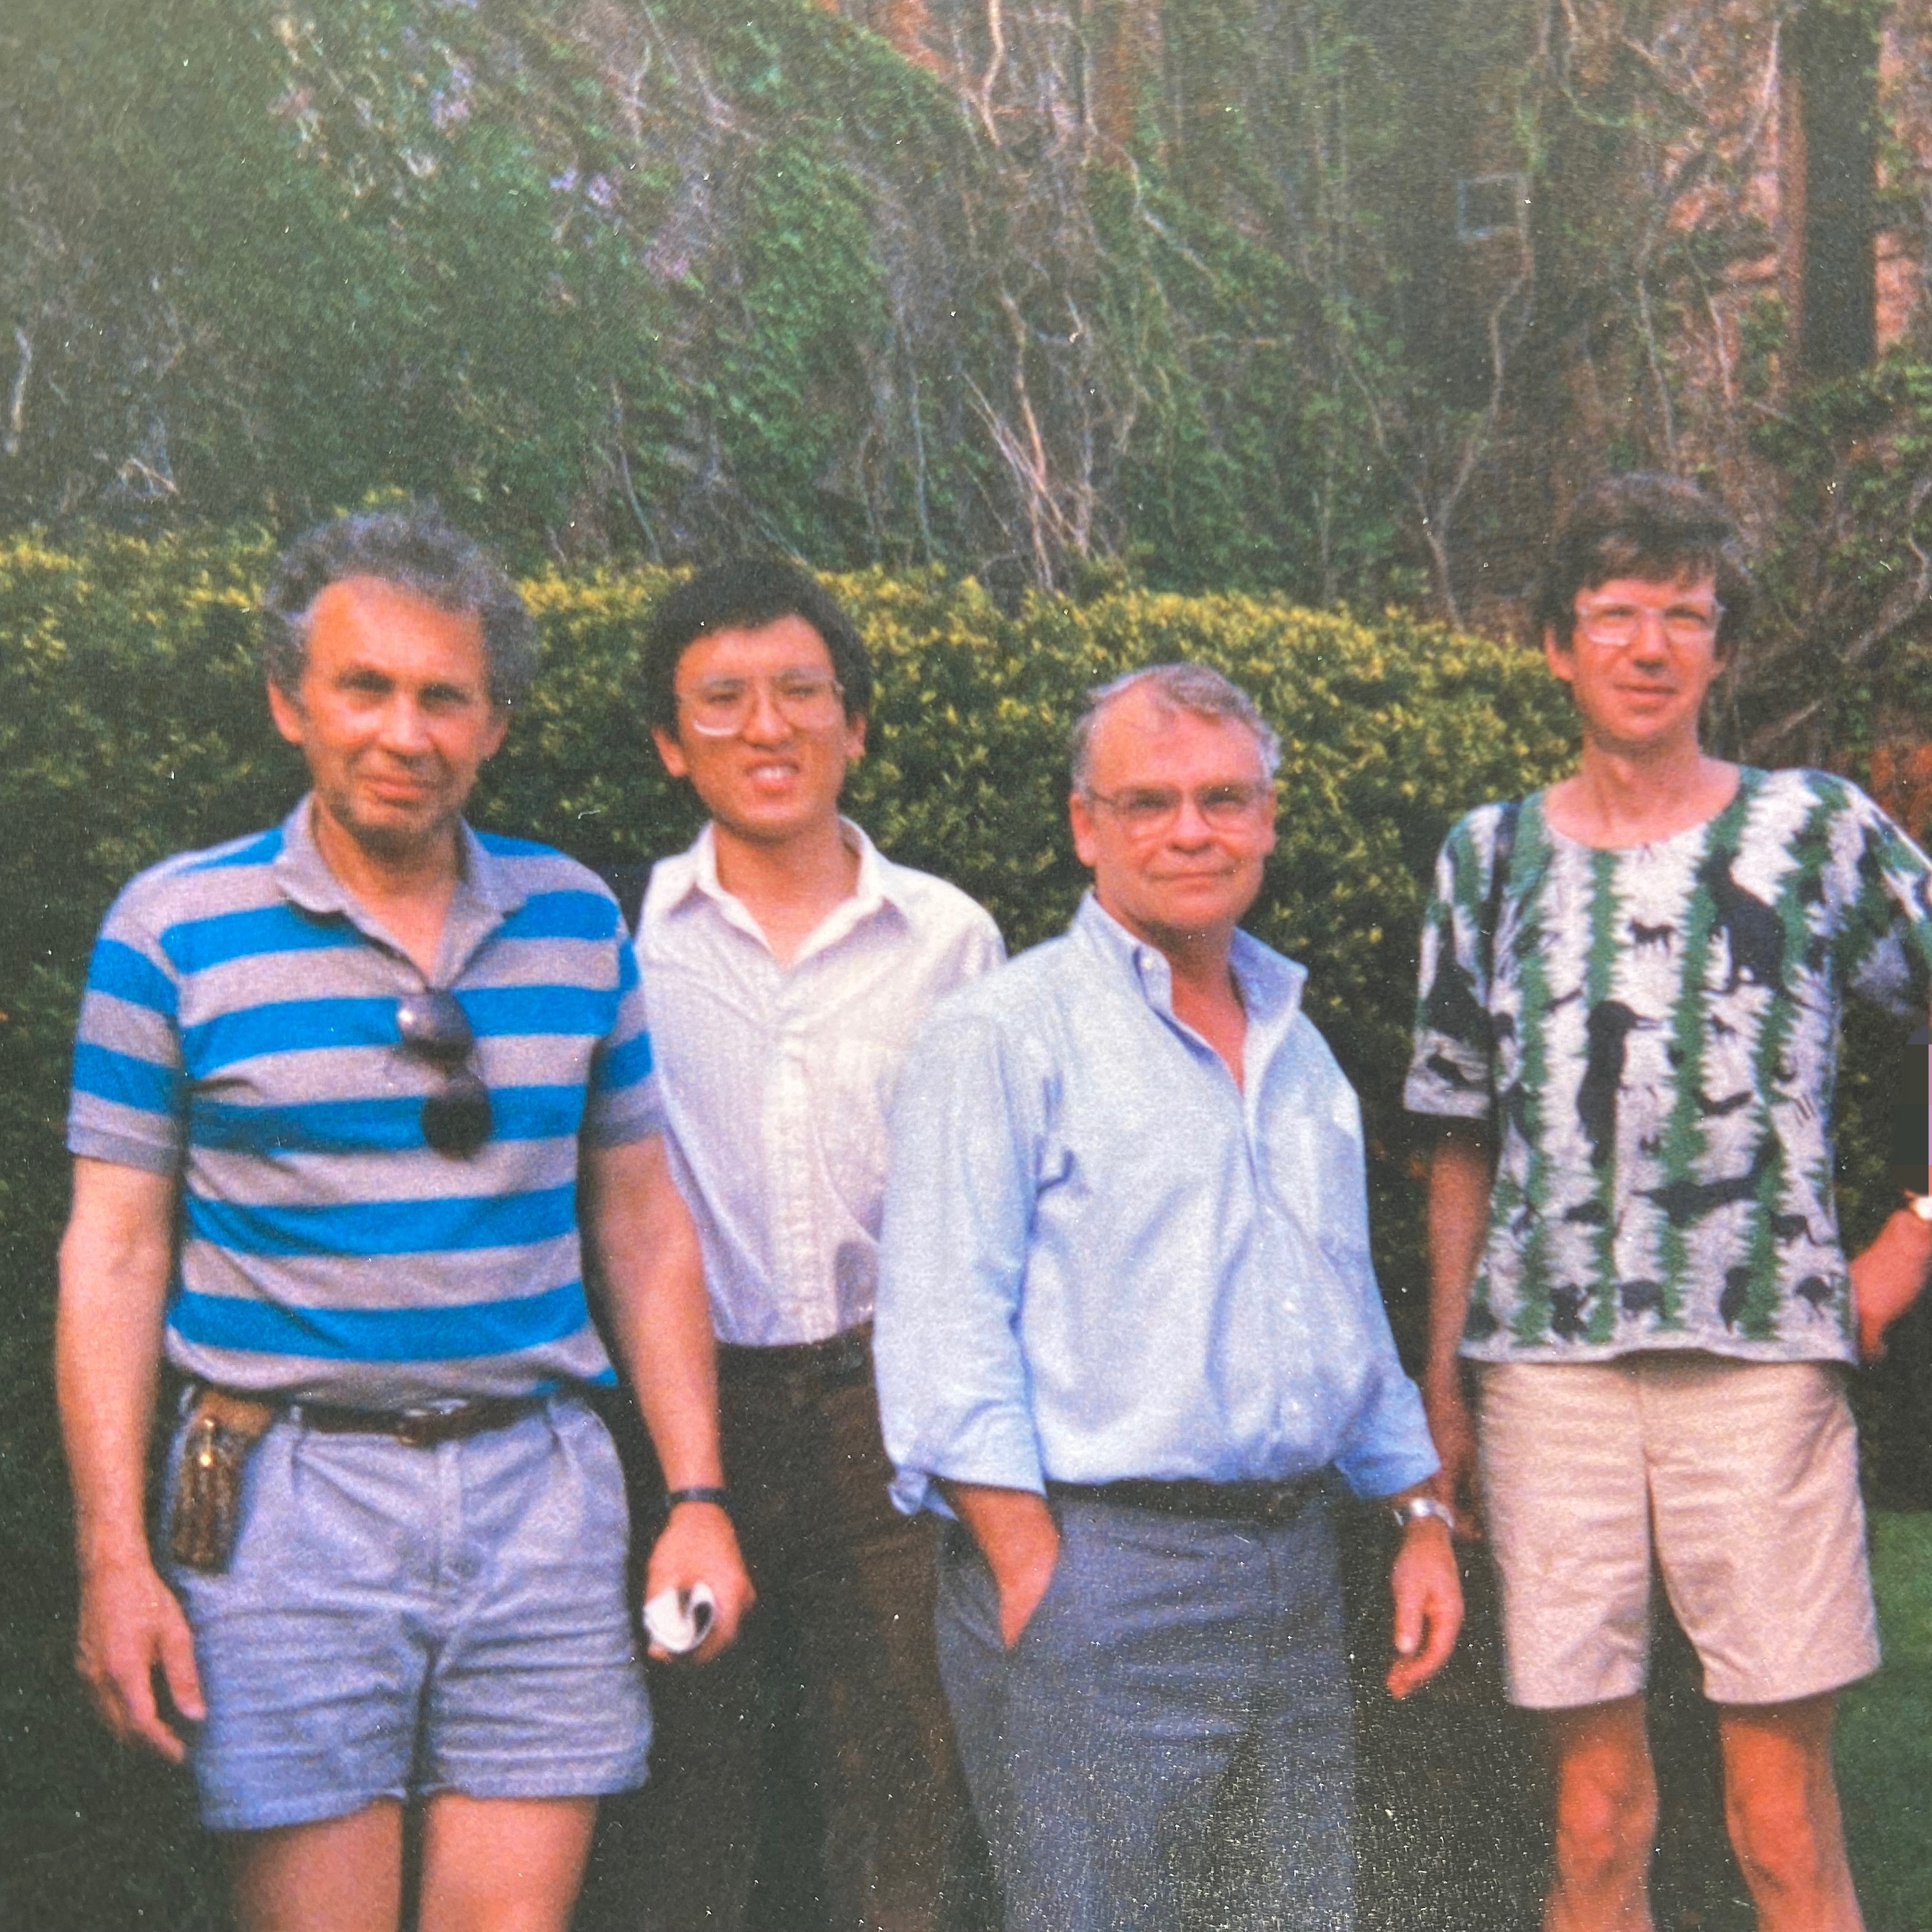
\includegraphics[height=2.5cm]{multigrid.org/photos-xu/BrambleSchatzWahlbinXu.jpg}
 \caption{\tiny From Left to right: Al, me, Jim and Lars}
 \label{Fig1}
\end{figure}
and Professor Vidar Thomee, a good friend of Jim, was a regular visitor. I was fortunate to interact frequently with these top numerical analysts. It was the best possible environment for a finite element researcher, nothing short of a dream come true. At that time, in particular, I worked closely with Jim, spending hours in his office discussing research problems. 

It was always amazing to me that Jim could discuss mathematics continuously for hours without so much as a short coffee break. A typical day started in his office around $9$ am, and we would talk until 3 or 4 in the afternoon. It was great to spend this time learning how to conduct research with him, but one thing really bothered me: Hunger! I typically skipped breakfast, so I often became very hungry, even to the point of feeling faint, during our discussions. But I was too afraid to say that I needed something to eat. Actually, I thought it impolite to eat in my boss's office. For some reason, Jim could go for hours and hours without eating yet remain highly energetic and engaged. I once asked him how he did it. His answer: a good breakfast. In all these years, though, I never did ask him what this miracle breakfast consisted of.
During our discussions, Jim would sit in front of his desk and I would stand at the whiteboard. From time to time, he would join me at my station and carry out derivation and calculations himself. In just this way, repeated day after day, Jim taught me how to conduct research and set the stage for me to become the independent researcher I am today. Jim loved doing research and he did it with great passion. Even after discussing a problem for hours, we would each go home and spend the evening working on any questions that remained. Whenever one of us made progress, we would eagerly go find the other to share the latest results and new ideas next day. It was so fun and so productive! Through this approach, Jim and I wrote eight papers together during my graduate days at Cornell.

I learned so much about conducting research from Jim. I remember well how in our early days working together, I would find Jim's insistence on staying with ideas that seemed to me hopeless to be quite (very!) annoying. After many, many attempts to make one of these ideas work, I would say something like ``Jim, this is not going to work. We should stop this and try something else.'' Oftentimes, he would respond ``No, no, no, let's try some more.'' I would think to myself, "This old man is out of his mind!" But more often than not, this persistence would lead to some interesting results. Even if the idea itself did not work, the process of working on it would lead us in new directions. Sometimes, for example, the idea could be applied to a different related problem.
There was both great productivity and great freedom in this approach. One of the nice things about mathematical research is that we work on interesting problems, but do not necessarily have to solve the problems we start with. If we end up solving entirely different problems, we are equally happy, and sometimes, Jim and I certainly did come up with better problems with beautiful answers. The creative freedom that can be found in conducting academic research is great, and is something that I first came to appreciate in my very earliest work with Jim.

Such a persistent and, in some sense, stubborn approach to research also means you can reasonably have confidence in your results. When another party suggests an idea you had already tried out before, you can confidently assert that it won't work and explain in depth why you know this to be the case. For this reason, I often ask my students these questions: "When you try an idea, do you know for sure that the idea won't work before you give up on it?" "If you obtain a new proof for a theorem, are you sure that your proof is correct and rigorous?" This is a matter of practice and maturity. Although you can not always be 100\% sure of any negative or positive conclusion, you can know that your conclusions have a very high probability of being correct. 
I learned this lesson the hard way. I had been trying to prove a result concerning the relationship between regularity and approximability. I had tried everything, or so I thought, but I just could not prove it. Eventually, I gave up. One day, though, I was in Jim's office, when a colleague called to talk about a new result he had heard about at a seminar. The result was exactly what I had been trying and failing to prove. So what had I missed? I started writing on the whiteboard to explain to Jim the approaches I had taken and why they had come up short. Amazingly, as I tried to explain the process, I hit on a simple new idea. A sudden revelation! I quickly wrote down a proof. Jim immediately confirmed it. That was quite an educational moment!

But, of course, things do not always work that way. For example, in 1988 or thereabouts, I wanted to establish a uniform weighted $L^2$ norm error estimate in terms of the corresponding weighted semi-$H^1$ norm. This result is critically important in establishing the uniform convergence of multigrid methods in respect to discontinuous jumps in the coefficient of the elliptic operator. I spent quite some time on this problem, but success eluded me. Again, Jim received a call while I was in his office: A colleague told him that another well-known mathematician and his student had announced that they had proved a uniform convergent result, similar to the one I had been trying to prove. Given my success in similar circumstances as described, I turned again to the whiteboard. Yet, this time, an hour passed with no progress to show for my effort. Many hours spent on the problem at home that evening advanced nothing. The lesson Jim had taught me was to keep on trying. And, indeed, I did. But this time, I took a different track: I began to wonder whether the result was actually correct. I started to think about a counter-example. Sure enough, shortly thereafter, I had produced a counter-example showing that the result was not and could not be right. The next day, I shared my progress with Jim, who confirmed that my example was, in fact, correct. Later, Jim encouraged me to write a paper on the subject, which I did (1991) \cite{xu1991counterexamples}. Further, I continued to work with Jim on weighted $L^2$ estimates and obtained a number of positive results on this topic. I am happy that we co-authored a paper in this area (1991) \cite{bramble1991some} and pleased that it has been cited in many research papers since. 

Jim served as an editor at the {\it Mathematics of Computation} journal for 25 years, where he also held the position of chief editor for 8 years. As an editor for this and other journals, Jim asked me to review numerous papers for possible publication, and I was glad to oblige. I read new papers with fresh perspectives from experts all over the world and found doing so to be a tremendous learning experience. I was thirsty for new research results such that I often read the papers overnight. I would ask Jim questions when I encountered difficulties, and I certainly learned a lot this way. I always tried to offer constructive suggestions and sometimes even new ideas or proofs for the result in the paper. This practice meant that from time to time, the authors would ask Jim for the name of the referee. He would always ask me if he could share my name, and I usually said OK. In the years since, I have had several interesting encounters with some of those authors. As just one example, at a conference in Japan sometime in the 1990s, a numerical analyst sought me out to tell me that based on my suggestions he had made significant improvements to his paper. 

\section{Jim took me to Circus and sent me to Penn State}
Jim was a co-founder (with Ivo Babuska and Bruce Kellogg) of the Finite Element Circus (established in 1970), which is a regular informal meeting devoted to the theory and applications of the finite element method and the related areas of numerical analysis and partial differential equations. During my time as a graduate student with Jim(spring 1985-fall 1988), he took me to every Finite Element Circus. I found it then as now to be a nurturing place for career development across generations. I have certainly been able to advance my own career through the Circus; in particular, it helped shape my research vision and set my career path as a graduate student and beyond. By attending the Circus, I learned about state-of-the-art results in finite element methods, took advantage of many opportunities to give talks on my own research results, and got to know many top researchers in finite element methods.

Among these researchers is L. Ridgeway Scott, who was a professor at Penn State at the time. My interactions with him at the Finite Element Circus determined my career path. One incident at the spring 1988 Circus held at Cornell changed my life. During the last talk, I happened to be sitting next to Ridg. When the organizer of the meeting announced that the Circus was now over, Ridg asked me a question of some consequence to my present and future: "How is it that you are always giving talks at the Circus, but haven't wrapped up your PhD yet?" Indeed, although I was beginning only my 4th year at Cornell at this time, I had already finished or started almost 8 papers with Jim and had also given many talks at the Circus. In response, I told Ridg that I very much enjoyed being at Cornell working with Jim and that we still had many problems to work on. But I also told him that I had visa problem. I was on a J1 visa, with a requirement to return to China within two years. This meant that I had no choice but to leave Cornell soon after I had finished my degree, as it would be almost impossible for me to secure an H1 visa after graduation. Upon hearing this, Ridg immediately invited me to apply for a position as a tenure-track assistant professor at Penn State, stating that we will help you solve that problem! I thought it was an incredible offer, and Jim agreed. "You go prepare a CV, and I'll write a good letter of recommendation." he said. I prepared a CV and asked Al and Lars to write letters of recommendation as well. I immediately sent my application to Penn State, and Jim, Al, and Lars quickly followed suit.  A couple of weeks later, Professor Richard Herman, head of Penn State's Department of Mathematics, called me. I heard him say, "I am making you an offer for a tenure-track assistant professor position at Penn State, starting next semester, fall 1988." I could hardly believe it. They had not even interviewed me for the job! I could only offer some puzzled and puzzling mumbling in response. "Right," he said, "I am making you this official offer without interviewing you, and I am also inviting you to visit Penn State as soon as possible to interview us. I very much hope you will accept our offer after your visit." These words sounded unbelievably kind to me, and I happily accepted the invitation for the visit which turned out to be overwhelming. Richard Herman and many colleagues in the department treated me so well. I quickly accepted the position providing that my visa problem could be resolved. 
During the visit, Ridg took me to the International Scholars Office, where the office director  told us that my visa problem could not be solved. Ridg and I returned to the department where Professor Herman countered "Oh, don't worry. We will fix it." A couple of weeks later, I received a letter from him with an airline ticket enclosed and a request to fly to Washington, DC, where he and Mr.~McQuaid, lead counsel for Penn State at the time, would meet me. As it turned out, Mr. McQuaid, at Herman's request, had engaged the best immigration lawyer he could find, namely, the former chief attorney for the US immigration office. The lawyer shared what proved to be critical expertise, including pointing to the need to obtain a strong endorsement for my visa application from an influential political figure, such as a senator or congressman. To my huge surprise, Herman managed to convince the university president to support me, who then convinced the legendary Penn State football coach Joe Paterno to contact then US Vice-President Bush to write a letter of endorsement for my visa application. I still cannot believe that he agreed to do so. In November 1988, Bush won the presidential election against Michael Dukakis. I, therefore, had the backing of the President-Elect of the United States of America. Thinking that this must surely mean I had a good chance of getting my visa problem resolved in my favor, I accepted the tenure-track position offer from Penn State, defended my thesis near the end of 1988 and started my career as an assistant professor at the institution's University Park Campus in spring 1989. Sure enough, my H1 visa came through in April 1989.

By any measure, the extraordinary efforts and steps that colleagues at Penn State took to ensure that a fresh PhD student could join their department are extremely overwhelming and flattering.  Till this day, I still cannot believe that I would get such an incredible treatment. I have no doubt that they acted based on what must have been a very generous recommendation from Jim—but then also from their own innate kindness and trust in me.   I am most grateful to Jim who made a special effort to take me as his student at Cornell,  trained me to do productive forefront research and his generosity in making the recommendation. 
I have had a very productive career so far and I love Penn State. I know that I would not have enjoyed this success without them.

\section{Jim wrote ten papers with me}
Jim made fundamental contributions to many topics in numerical methods for partial differential equations and has more than 200 papers to his credit. Although best known for his seminal work in finite element methods, he also made fundamental contributions to the theoretical analysis of finite difference methods in the 1960s. One of his most famous results is the Bramble-Hilbert Lemma, which has become a basic tool in the error analysis of functional space consisting of piecewise polynomials such as finite element methods. Further, Jim also made fundamental contributions to the design and analysis of domain decomposition methods and multigrid methods for the solution of algebraic systems arising from the discretization of elliptic and parabolic problems. 
My own publications record includes ten papers written in collaboration with Jim \cite{bramble1988analysis,bramble1989local,bramble1990parallel,bramble1991analysis,bramble1991convergence-a,bramble1991convergence-b,bramble1991some,bramble1992multilevel,bacuta2003regularity-a,bacuta2003regularity-b} as shown below:

\begin{enumerate}
\item	Bramble, J.H., Pasciak, J.E., Xu, J. (1988). The analysis of multigrid algorithms for nonsymmetric and indefinite elliptic problems. Mathematics of Computation, 51(184), 389-414. Google Scholar Citations: 109.
\item	Bramble, J.H., Xu, J. (1989). A local post-processing technique for improving the accuracy in mixed finite-element approximations. SIAM journal on numerical analysis, 26(6), 1267-1275. Google Scholar Citations: 50.
\item	Bramble, J.H., Pasciak, J.E., Xu, J. (1990). Parallel multilevel preconditioners. Mathematics of Computation, 55(191), 1-22. Google Scholar Citations: 1023.
\item	Bramble, J.H., Pasciak, J.E., Xu, J. (1991). The analysis of multigrid algorithms with nonnested spaces or noninherited quadratic forms. Mathematics of Computation, 56(193), 1-34. Google Scholar Citations: 310.
\item	Bramble, J.H., Pasciak, J.E., Wang, J.P., Xu, J. (1991). Convergence estimates for multigrid algorithms without regularity assumptions. Mathematics of Computation, 57(195), 23-45. Google Scholar Citations: 389.
\item	Bramble, J.H., Pasciak, J.E., Wang, J.P., Xu, J. (1991). Convergence estimates for product iterative methods with applications to domain decomposition. Mathematics of Computation, 57(195), 1-21. Google Scholar Citations: 385.
\item	Bramble, J.H., Xu, J. (1991). Some estimates for a weighted $L^2$ projection. Mathematics of Computation, 56(194), 463-476. Google Scholar Citations: 330.
\item Bramble, J.H., Pasciak, J.E., Xu, J. (1992). A multilevel preconditioner for domain decomposition boundary systems. Mathematical Sciences Institute, Cornell University 92(27). Google Scholar Citations: 9.
\item Bacuta, C., Bramble, J.H., Xu, J. (2003). Regularity estimates for elliptic boundary value problems with smooth data on polygonal domains. Journal of Numerical Mathematics, 11(2), 75-94. Google Scholar Citations: 29.
\item Bacuta, C., Bramble, J., Xu, J. (2003). Regularity estimates for elliptic boundary value problems in Besov spaces. Mathematics of Computation, 72(244), 1577-1595. Google Scholar Citations: 59.
\end{enumerate}
Eight of the ten papers on which I partnered with Jim were started and/or finished while I pursued my graduate work under his guidance. I wrote two more papers with Jim and his PhD student Constantin Bacuta when Constantin became a postdoctoral fellow with me at Penn State immediately after he had finished his own doctoral degree. Jim was instrumental in helping me quickly find my place in the forefront of research fields including finite element, domain decomposition, and multigrid methods. In fact, although I have published more than 200 papers, those that Jim and I worked on together are and will always be among the most important publications of my career.
My joint papers with Jim were mostly written while I was a graduate student with him. Through his special way, Jim trained his PhD students to become independent researchers so that although his research continued to influence me, I became an independent researcher soon after leaving Cornell in 1989. %Ever since and still today, I try to emulate this approach with my own students. 

I recently created \href{https://scholar.google.com/citations?user=RuZVUoAAAAAJ\&hl=en\&oi=ao}{a Google Scholar profile for Jim}.
Listed here are his ten most highly cited papers according to Google Scholar analytics (I am happy to see that I am a co-author on five papers of these!). 
\begin{enumerate}
\item Bramble, J.H., Pasciak, J.E., Xu, J. (1990). Parallel multilevel preconditioners. Mathematics of Computation, 55(191), 1-22. Google Scholar Citations: 1022. 
\item Bramble, J.H., Pasciak, J. (1988). A preconditioning technique for indefinite systems resulting from mixed approximations of elliptic problems. Mathematics of Computation, 50(181), 1-17. Google Scholar Citations: 589.
\item Bramble, J.H., Hilbert, S.R. (1970). Estimation of linear functionals on Sobolev spaces with application to Fourier transforms and spline interpolation. SIAM Journal on Numerical Analysis, 7(1), 112-124. Google Scholar Citations: 550.
\item Bramble, J.H., Pasciak, J.E., Vassilev, A.T. (1997). Analysis of the inexact Uzawa algorithm for saddle point problems. SIAM Journal on Numerical Analysis, 34(3), 1072-1092. Google Scholar Citations: 534.
\item Bramble, J.H., Pasciak, J.E., Wang, J.P.,  Xu, J. (1991). Convergence estimates for multigrid algorithms without regularity assumptions. Mathematics of Computation, 57(195), 23-45. Google Scholar Citations: 389.
\item Bramble, J.H., Pasciak, J.E., Wang, J.P., Xu, J. (1991). Convergence estimates for product iterative methods with applications to domain decomposition. Mathematics of Computation, 57(195), 1-21. Google Scholar Citations: 385.
\item Bramble, J.H., Hilbert, S.R. (1971). Bounds for a class of linear functionals with applications to Hermite interpolation. Numerische Mathematik, 16(4), 362-369. Google Scholar Citations: 367.
\item Bramble, J.H., Xu, J. (1991). Some estimates for a weighted $L^2$ projection. Mathematics of Computation, 56(194), 463-476. Google Scholar Citations: 330.
\item Bramble, J.H., Schatz, A.H. (1977). Higher order local accuracy by averaging in the finite element method. Mathematics of Computation, 31(137), 94-111. Google Scholar Citations: 328.
\item Bramble, J.H., Pasciak, J.E., Xu, J. (1991). The analysis of multigrid algorithms with nonnested spaces or noninherited quadratic forms. Mathematics of Computation, 56(193), 1-34. Google Scholar Citations: 310.
\end{enumerate}
I had a look at my own publications record and and found that five of my ten most cited papers were co-authored with Jim:
\cite{xu1992iterative,bramble1990parallel,xu1996two,xu1994novel,bramble1991convergencea,bramble1991convergenceb,bramble1991some,hiptmair2007nodal,bramble1991analysis,xu1998some}. 

Evidently, the papers I wrote with Jim represent a significant part of my scientific work. I still remember the first project that Jim gave me to work on: It involved trying to establish a uniform multigrid convergence theory for the elliptic boundary problem, which has a coefficient with sharp discontinuous jumps across two subdomains. This was sometime in 1995, the first year of my life as a graduate student at Cornell. At the time, the multigrid convergence theory depended on the elliptic regularity theorem, which does not hold (uniformly) for PDE with sharp discontinuous coefficients. This is a tough problem—and also an extremely important one. For two or three years, I tried to solve it, eventually succeeding towards the end of my graduate study at Cornell in a joint work with Jim, J. Pasciak, and J. Wang~\cite{bramble1991convergence-a}. But, during my work on this first research project, we also obtained a number of important results related to this basic question, including results on weighted $L^2$ projections, which are related to what is referred to as the Bramble-Pasciak-Xu (BPX) preconditioner \cite{bramble1990parallel}. In BPX theory, we did not use elliptic regularity theory (modular a logarithmic factor). BPX turned out to be one of two fundamental multigrid algorithms for solving the elliptic boundary problem, the other is the class V-cycle multigrid algorithm. BPX can be viewed as a parallel version of the classic V-cycle. Based on these works, I later formulated an abstract framework in \cite{xu1992iterative}, which classifies most iterative methods into two types: successive and parallel subspace correction methods. I am so thankful to Jim for giving me such a meaningful problem to begin my research with him and for sharing with me the great vision and depth of his work and overall approach to research, teaching and, of course, advising. 
\section{Jim as a father figure}
My four years at Cornell were of great importance to my professional career, but also in relation to my personal life. It was at Cornell where I met my wife, Jenny Li, a graduate student in mathematics as well as economics and today also a faculty member with Penn State's Department of Mathematics.
While I certainly made progress in my research at Cornell, I was definitely not well-prepared, either emotionally or socially, to live in a new country with a new language. I've had many dramatic changes in my life. I was born and raised in a poor family in the Chinese countryside. My parents were both illiterate. I was the only one in my village to go to college in 1978. The transitions I made from a poor and innocent country boy to become a college student at Xiangtan University and then a graduate student at Peking University were exciting and challenging, but also daunting. My transition from China to the US, specifically from Peking University to Cornell University, was definitely the biggest change. I got lost in a new country, a new culture, a new language, and a new environment. The extremely cold weather in Ithaca that greeted me on my arrival in early spring 1985 didn't help! Jim encouraged and helped me at every stage during this period from day one and then ever after. 

Jenny, and I married in August 1988. We got a lot advice from Jim while we prepared for the big day. He jokingly told us that: "I have a lot of experience planning weddings. I myself have been married twice and I also helped organize the weddings for my daughters and sons. So you can ask me any question on how to prepare for a wedding."
Jim and his wife, Peggy, also hosted a wonderful bridal shower for us shared by many cherished colleagues and friends. Our parents could not attend our wedding, so Jim walked Jenny down the aisle. He also gave a wonderful speech, which he ended in Chinese: "你是我的好朋友 (You are my good friends) (see Fig. \ref{FigW})."  It was so touching.
\begin{figure}[h]
 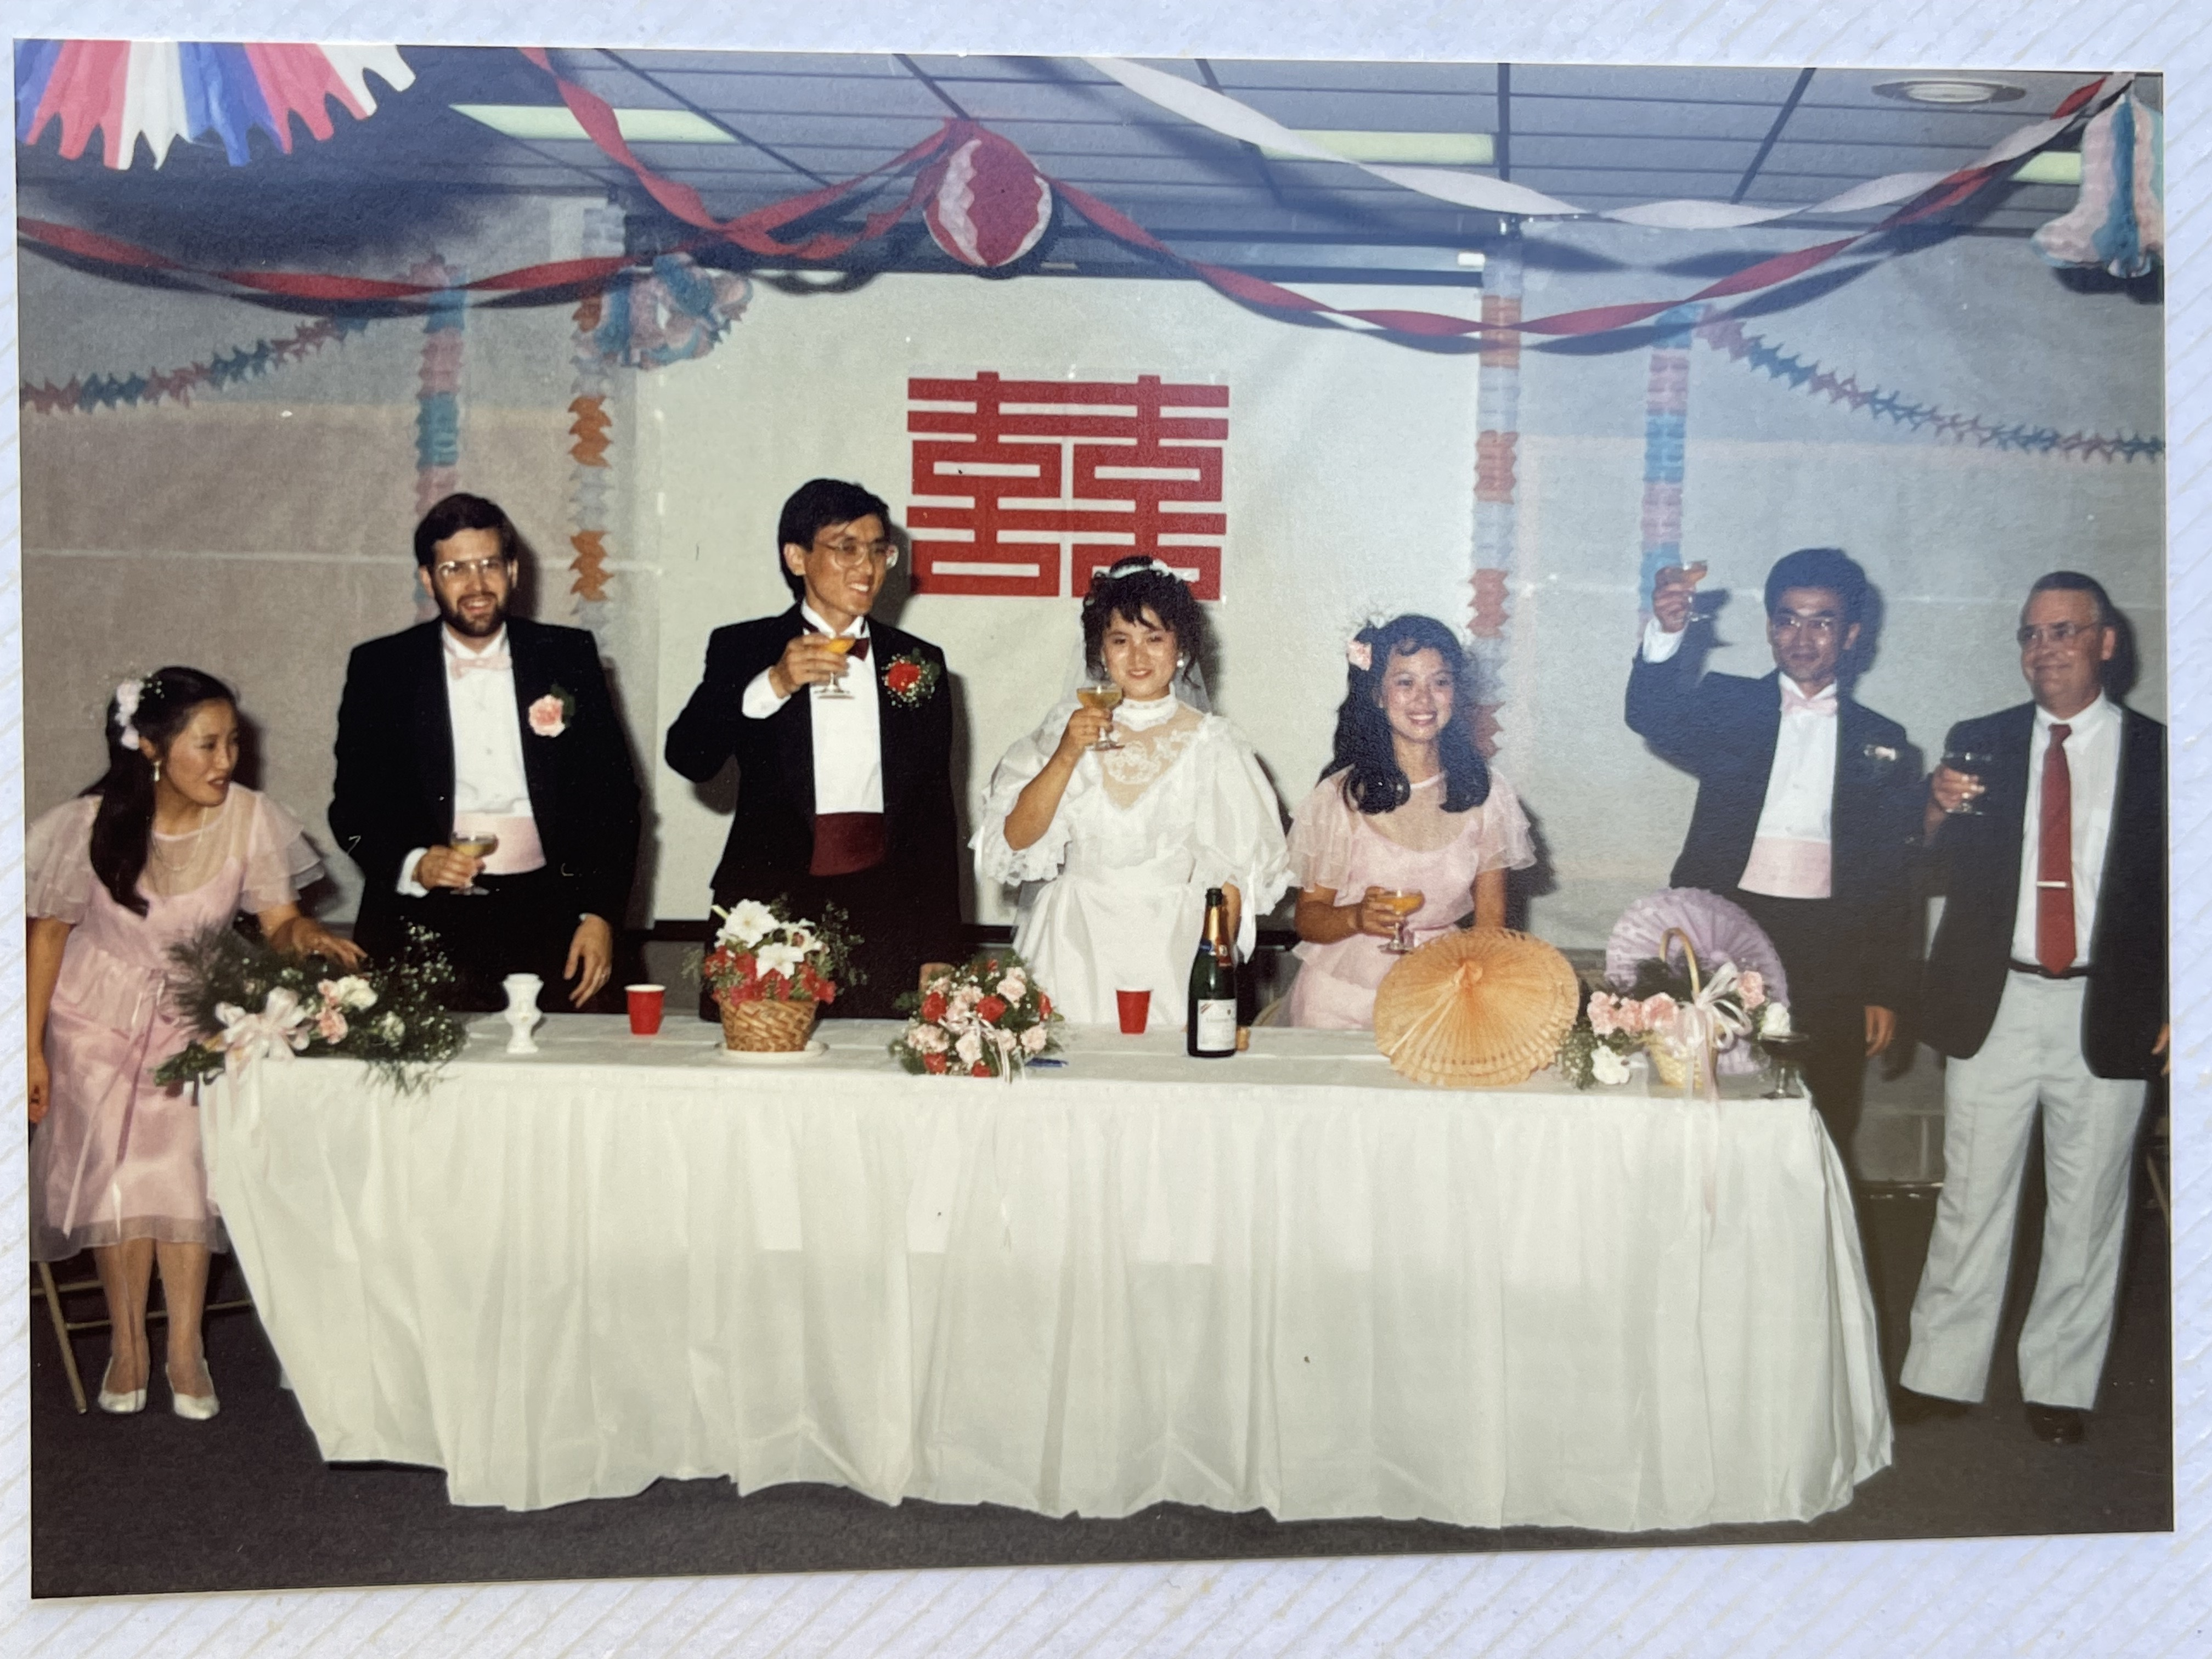
\includegraphics[height=2.5cm]{multigrid.org/photos-xu/Jim@Wedding.jpeg}
 \caption{\tiny Jim attending my wedding}
 \label{FigW}
\end{figure}

\section{Last meetings}
After Jim retired from Texas A\&M, I visited him several times at his home in Austin. My last visit was in February 2020. I contacted Mary Wheeler, a neighbor and good friend of Jim to facilitate it. After consulting with Jim's son, Jay, Mary and I went to Jim's favorite local place, the County Line Restaurant, to buy his favorite foods. I also bought a good bottle of red wine, the very best I could get in the city of Austin. Mary and I went to Jim's house with the food and wine. He was very happy to see us. Jim had a nurse by this time and greeted us from his wheelchair. He cheerfully greeted us both, and we had a great conversation and a wonderful lunch together. He always did enjoy a good bottle of wine, and I was happy to filled his wine glass. In fact, he drank several glasses! I remembered that I had also brought wine during my last visit. Peggy was still alive then and the three of us had enjoyed a great time together. This time, Peggy was no longer with us. It was saddening to miss her. She, too, was an exceptionally kind and insightful person, a great match for Jim, and dear friend to both Jenny and me in so many ways. 
\begin{figure}[h]
 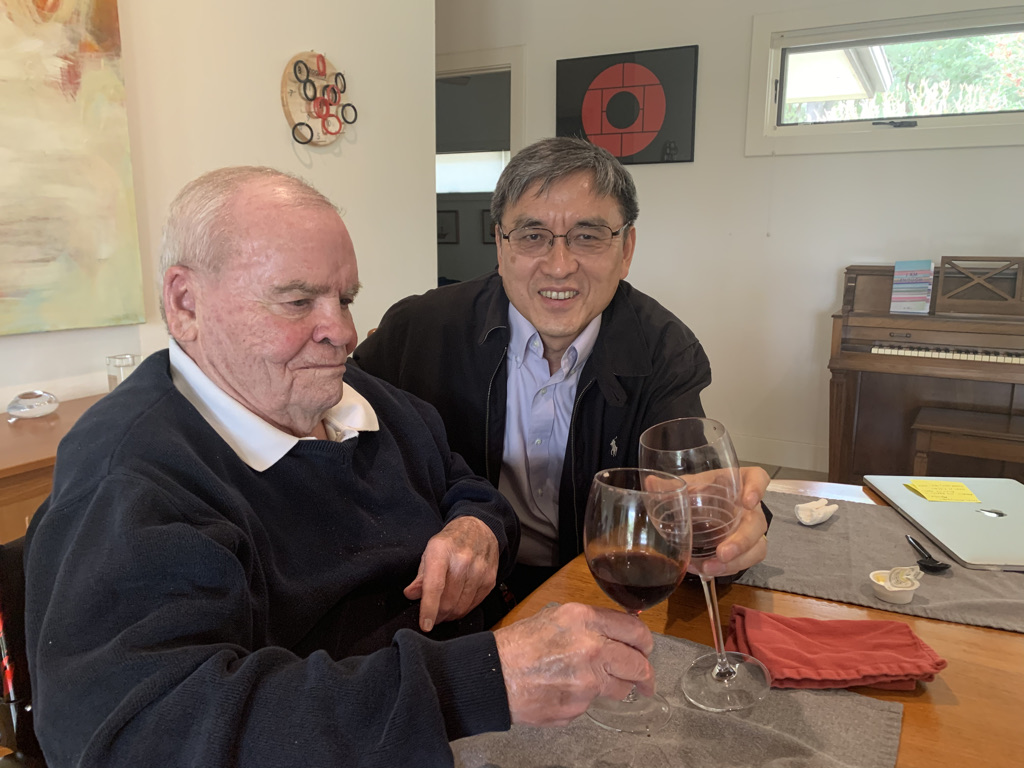
\includegraphics[height=2.5cm]{multigrid.org/photos-xu/VisitJimHome20200224/JimJinchao20200224.jpeg}
 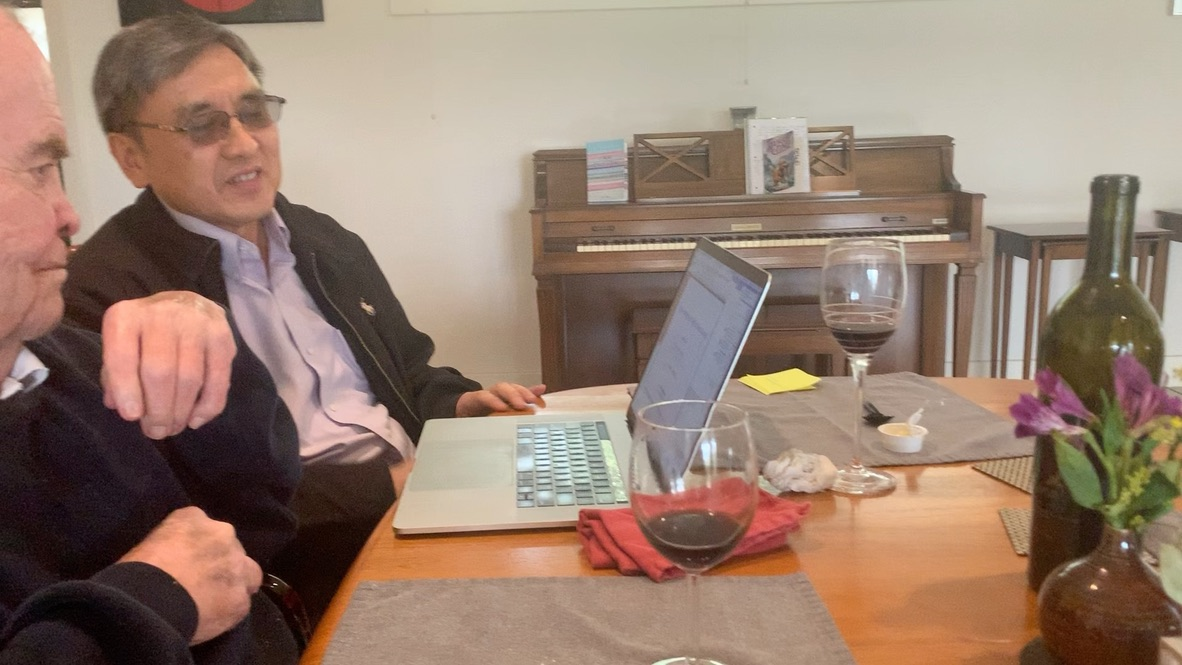
\includegraphics[height=2.5cm]{multigrid.org/photos-xu/VisitJimHome20200224/Convolution20200224.jpeg}
 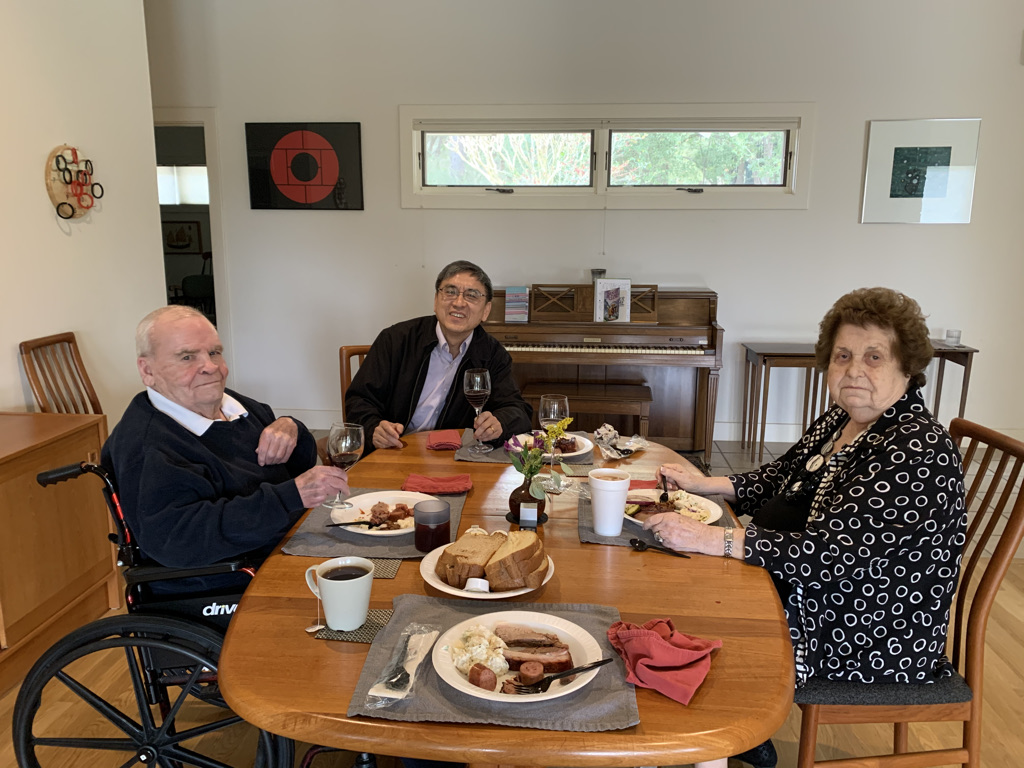
\includegraphics[height=2.5cm]{multigrid.org/photos-xu/VisitJimHome20200224/JimMaryJinchao20200224.jpeg}
 \caption{\tiny Left: a toast with Jim; middle: discuss math; right: with Jim and Mary}\label{Fig2}
\end{figure}
My very last meeting with Jim was through Zoom. It was during the 50th Anniversary Finite Element Circus Meeting (November 2020). During the Circus, I contacted Jim's son, Jay, and asked him if he could get his Dad online. Jim joined us on Zoom and shared conversations with many of his former students, colleagues, and friends. It was such a nice moment. We celebrated the success of the Finite Element Circus that he had helped to start with Ivo Babuska  and Bruce Kellogg.  Ivo was also present to create this unforgettable time shared together.
\section{Last words}
Jim has now left us forever. I hope he rests in peace. I am so grateful for everything he has done for me. I do my best to share his wisdom with others. I miss him greatly. 
\bibliographystyle{plain}
\bibliography{ArticleCollection/bramble.bib,XuPublications.bib}
\end{CJK*}
\end{document}


Links:

* Announcement [Cornell]

* Memories and Condolence

* Jim's Students:   The Life and Mathematics of Jim Bramble 

* Jinchao Xu:  In Loving Memory of My Great Mentor and Friend, Dr. Jim Bramble

* The Collected Works of James H. Bramble

* Photos





